\section{Overview}\label{subsec:overview}
\bruno{Summary of the Section must come first. Look at the
  ``Extensibility for the Masses'' to see how sections are written.}
In this section, we start by considering a practical problem of representing tree structure in simple object-oriented approach. It turns out that this approach of coding is lengthy and lacks extensibility when the tree structure is big in size. We then applies object algebras to help solving extensibility problem, but the code is still full to tedious delegation code in the tree structure nodes. Thus we introduce generic queries and transformations to make traversal code reusable and modular. Finally we present our framework \name which automatically generate generic queries, generalized generic queries, transformations and contextual aware transformations based on Object Algebra Interfaces with Java annotation.

\subsection{Object Oriented Solution}
We start by considering the company structure introduced in
Fig.~\ref{company_structure}.\bruno{More text needed. Where does the
company example come from? add a reference to it.} This example is borrowed from \cite{ralf03syb}, where they use the example to address the problem of boilerplate code when programming with rich tree structures in Haskell. 

\begin{figure}[ht!]
\centering
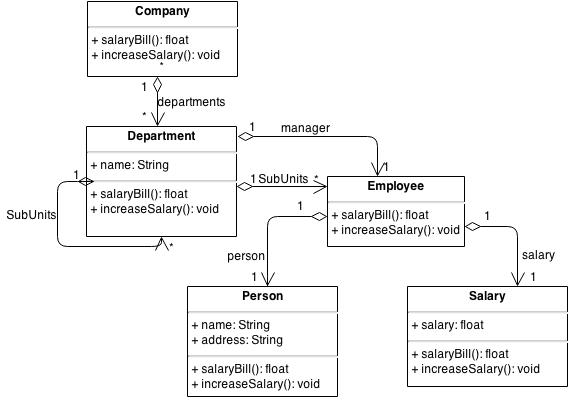
\includegraphics[width=90mm]{Company.jpg}
\caption{Company Structure \label{company_structure}}
\end{figure}

A very natural Object-Oriented way to model the company structure is
as illustrated in Figure~\ref{oop_company}. Similar code can be applied to
\lstinline{Department}\bruno{references to code identifiers should be
  printed with code font as in \lstinline{Department}.Change all such 
references throughout the paper.},
\lstinline{Employee}, \lstinline{SubUnit} and \lstinline{Person}. A Company comprises a list of
Departments. Each Department is managed by an Employee as the manager
and contains a list of SubUnits. The SubUnit can be either a
department or an Employee. An Employee is a Person with the Salary
Information.

\begin{figure}[tb]
\lstinputlisting[linerange=6-23]{../ObjectAlgebras/src/sybDemo1/Company.java} % APPLY:linerange=OOP_COMPANY
\vspace{-.1in}
\caption{Company Class in OOP style}
\label{oop_company}
\end{figure}
\bruno{No need for 2 figures. Just put the code for the
  two classes in a single figure.}

Now consider adding two operations to our company structure: query the
salary bill for the whole company and increase the salary of each
employee by 10\%. A very natural solution, as illustrated in Fig.~\ref{oop_company}, is to add methods \lstinline{Float salaryBill()} and \lstinline{void increaseSalary()} in all classes from the bottom \lstinline{class Salary} to the top \lstinline{class Company}, except some sibling classes like \lstinline{class Person} which has nothing to do with salary information. Thus query salary bill of the whole company can be implemented as return the salary in \lstinline{class Salary} and delegating the method \lstinline{Float salaryBill()} to the child leaves for the upper level classes in the company tree structure, while increase salary of the whole company by 10\% can be implemented by updating the salary information in \lstinline{class Salary} and delegating the method \lstinline{void increaseSalary()} to the child leaves for the upper level nodes.  \bruno{Some more text
  needed: why do we need to have the methods in most classes, but not
  in \lstinline{Person}?}

However, this simple object-oriented solution is lack of extensibility and with large amount of boilerplate code when traversing the tree structures. 

\begin{enumerate}

\item {\bf Lack of extensibility} \bruno{explain}
This way of Object Oriented style representation of tree structures can become cumbersome and inflexible due to the bound relationship between classes. For instance, adding another layer of nodes between classes, such as adding a class Team in our Company example, requires modifying its parent classes and child classes, which violates the no modification rule and are prone to errors. Adding a new operation such as pretty printing of the company structure requires adding a lot of similar methods on the existing code and violates the no modification rule.

\item {\bf Boilerplate code} \bruno{explain}
Another issue of the above solution is that we usually need to write a large amount of boilerplate code to implement very simple task. In our example, we implemented \lstinline{void increaseSalary()} and \lstinline{Float querySalary()} in almost all classes, while only \lstinline{class Salary} does some interesting work, other classes simply delegating the task to its child nodes. This problem become more severe when we have bigger tree structures. The useful code can become very little while most of the code is doing tedious delegation work. 

\end{enumerate}

\bruno{The following text needs to be stronger (use the template
  above) to better emphasize the two problems that arize here.}



\subsection{Modeling Company Structure with Object Algebras}

To tackle with the problem of extensibility, Object Algebras is a good solution. \bruno{text missing here. We need to introduce object algebras first; explain what they are; cite them; and then talk about the solution.} Oliveira proposed the design pattern \emph{Object Algebras}\cite{bruno12oa} to solve the famous Expression Problem. Object Algebras are classes that implement Object Algebra Interfaces where the type parameters represents the algebra classes. With this extra layer of generic type parameters, Object Algebras is extensible on both data variants and operations.  

\begin{figure}[tb]
\lstinputlisting[linerange=8-17]{../ObjectAlgebras/src/trees/SybAlg.java} % APPLY:linerange=SYB_TREE
\vspace{-.1in}
\caption{Company Structure represented by Object Algebra Interface}
\label{syb_tree}
\end{figure}

Fig.~\ref{syb_tree} shows the approach to model the Company
structure as an object algebra interface. Different operations can be realized by extending object algebras inheriting from the object algebra interface. To implement query bill
operation for the whole Company structure, we can implement the
Company interface with specific operation for each component.

\begin{lstlisting}[numbers=none] 
public class QuerySalarySybAlg implements SybAlg<Float,Float,Float,Float,Float,Float> {
	public Float C(List<Float> depts){
		Float r = 0f;
		for (Float f: depts) r += f;
		return r;
	}
	...
	public Float S(float salary){
		return salary;
	}
}
\end{lstlisting}

While IncreaseSalary can be realized as: 

\begin{lstlisting}[numbers=none]
public class IncreaseSalarySybAlg implements SybAlg<Float, Float, Float, Float, Float, Float> {
	public SybAlg<Float, Float, Float, Float, Float, Float> alg;
	public IncreaseSalarySybAlg(SybAlg<Float, Float, Float, Float, Float, Float> alg) { this.alg = alg; }
	public Float C(List<Float> depts) {
		return alg.C(depts);
	}
	...
	public Float S(float salary) {
		return alg.S(salary*1.1f);
	}
}
\end{lstlisting}\bruno{The code is too specific. It should be
  something like: \lstinline{public class
    IncreaseSalarySybAlg<Company, Dept, SubUnit, Employee, Person,
    Salary> implements SybAlg<Company, Dept, SubUnit, Employee,
    Person, Salary>}}

\bruno{code needs to be better explained. What are we using the
  \lstinline{alg} for?}
  
We pass in Float as type parameter class to represent salary. Hence different operations, i.e. query salary bill and increase salary of the company, can be done with inheritance. When programming with Object Algebras, the code can be very generic based on the object algebra interfaces. \lstinline{alg} can be used as an abstract factory to construct algebras, while the algebras can be instantiated by specific object algebras later by passing in type parameters. 

However, although we solved the problem of extensibility with object algebras, the traversal code is still lengthy and we are writing tedious boilerplate code. The only code we are really interested in is the \lstinline{Salary S(Float salary)} method to return or to increase the salary. It will be better if we can design some generic classes for queries and transformations. Hence specific algebras can be generated by
implementing interesting cases of generic queries and
transformations. Moreover, it will be even better if the boilerplate code can be generated automatically so we can focus our attention on the interesting cases.

\subsection{Object Algebra Framework}
Motivated by this problem of writing generic code for tree structure
traversals, we introduce generic queries, generalized generic queries, transformations and contextual aware transformations with Object Algebras, which can be easily inherited by real cases of queries and transformations. Furthermore, we designed an object algebra framework \name. With our framework, the generic query and transformation classes can be generated automatically by adding an ``$@$Algebra'' annotation.

Now with our Object Algebra Framework, the code we need to write for Salary Bill and Increase Salary will be much shorter. A Generic query code will be as short as Fig.~\ref{query_with_oaframework}. Here when coding with the framework \name, users need not worry about any boilerplate delegation code of the tree structure, but just simply rewrite the interesting case which actually return the salary information.
\begin{figure}[tb]
\lstinputlisting[linerange=8-11]{../ObjectAlgebras/src/example_SybAlg/FloatQuery.java} % APPLY:linerange=QUERY_WITH_OAFRAMEWORK
\vspace{-.1in}
\caption{Query Salary Class with Object Algebra Framework}
\label{query_with_oaframework}
\end{figure}


Transformation code will be like Figure~\ref{transform_with_oaframework}. Similar to the query example, all the boilerplate part has been handled by the framework and the developer only needs to pass in the original company algebra and override the interesting case \lstinline{Float S(float salary)}, then a new company algebra will be returned after transformation.  
\begin{figure}[tb]
\lstinputlisting[linerange=7-12]{../ObjectAlgebras/src/example_SybAlg/IncSalary.java} % APPLY:linerange=TRANSFORM_WITH_OAFRAMEWORK
\vspace{-.1in}
\caption{Increase Salary Class with Object Algebra Framework}
\label{transform_with_oaframework}
\end{figure}

\bruno{code is too specific. See comment about previous
  increase salary example}
\begin{comment}The classes SybAlgQuery<R>, SybAlgTransform<R,R,R,R,R,R> are generated
by the framework automatically. \end{comment}
\bruno{Jason, generally speaking your explanations of the code are to
  brief: you don't actually explain the code. You need to emphasize
  the relevant parts of the code, as well as the parts that are
  non-obvious. Here for example you want to emphasize that we only
  need to write the salary method.}